\documentclass[12pt,a4paper]{article}


%----------------------------------------------------------------------
% PACKAGES AND BASIC SETUP
%----------------------------------------------------------------------
\usepackage[utf8]{inputenc}        % For UTF-8 encoding
\usepackage[T1]{fontenc}           % For proper accented characters
\usepackage{lmodern}               % Latin Modern font
\usepackage{geometry}              % Adjust page margins
\geometry{margin=1in}             % 1-inch margins all around
\usepackage[backend=bibtex]{biblatex}  
\addbibresource{sample.bib}  
\usepackage[margin=1in]{geometry}
\usepackage{amsmath}
\usepackage{url}
\usepackage{hyperref}
\usepackage{titlesec}
\usepackage{enumitem}
\usepackage{fancyhdr}
\usepackage{caption}
\usepackage{setspace}              % For line spacing if needed
%\onehalfspacing                    % Uncomment for 1.5 spacing
\usepackage{multirow} % Add this to the preamble
\usepackage{caption}

\usepackage{graphicx}              % For including images
\usepackage{hyperref}              % Clickable links in PDF
\usepackage{amsmath,amssymb}       % Math symbols if needed
\usepackage{parskip}               % Blank line between paragraphs
\usepackage{float}
\usepackage{xcolor}
% If you want MLA or APA style references, you can use biblatex or natbib
% e.g.:
%----------------------------------------------------------------------
% TITLE PAGE INFO
%----------------------------------------------------------------------
\title{

    \rule{\textwidth}{4pt}\\[10pt]
    \huge \textbf{Data Engineering Project Report}
    \rule{\textwidth}{1pt}\\[15pt]
    
    \huge \color{darkgray}\textbf{StarGazers Predictor: GitHub Stars Prediction Pipeline}\\[15pt]
    
    \large \textbf{Department of Information Technology}\\[15pt]
    \large \textbf{By Group 2}\\[5pt]


}
\author{
    Shaheryar\\
    \texttt{shaheryar.4822@student.uu.se}
    \and
    Rick\\
    \texttt{riccardo.rebecchi.8372@student.uu.se}
    \and
    Feruz\\
    \texttt{@student.uu.se}
    \and
    Lu\\
    \texttt{lu.chen.9450@student.uu.se}
    \and
    Linjia\\
    \texttt{@student.uu.se}
    }
\date{\today} % Updates Daily


\begin{document}

\maketitle

\section{Introduction}
This project proposes and implements a complete "Star Predictor" system. The system collects historical data of open source projects through the GitHub API, extracts key features of the project activity (such as repository size, ammount of folks, etc.), trains multiple machine learning models (XGBoost, random forest, etc.), and selects the best model based on the prediction accuracy to achieve modeling and prediction of the popularity of open source projects. We use two virtual machines (VMs) for system deployment, one for model development and training, and the other for production deployment, and use GitHooks to achieve continuous integration and delivery of the model. Finally, the deployed application can predict and rank 5 GitHub projects, simulating the actual application scenario of the recommendation system.

This study finally verified the differences in prediction accuracy among different models, and also evaluated the scalability and practicality of the overall system.

\section{Related Work}
Early research treated GitHub stars as a direct indicator of repository popularity and explored simple predictive models. For example, Borges et al.\cite{3} applied multiple linear regression to forecast the number of stars a repository might receive. They found that incorporating recent project activity significantly improved accuracy, and their models performed best when trained on data from the last six months of activity. 

Subsequent studies have explored this topic using more advanced methods and broader datasets. A study by Han et al. (2019) conducted a large-scale study of over 400,000 repositories to classify which projects would cross a popularity threshold of 100 stars. They collected 35 different features about each repository, including development activity, using a random forest classifier, their model achieved strong results and identified development activity as a key predictor of success.\cite{1}  

Another relevant study was carried out by Sahin et al. (2019),\cite{4} who used recurrent neural networks to model GitHub popularity as a time-series prediction task. Their model incorporated key metrics like commits, forks, releases, and contributor information, with additional weighting based on user influence. The study demonstrated that development activity and user engagement features are valuable inputs for forecasting future popularity. Ren et al.\cite{2} proposed a model called StarIn, which combines traditional repository activity features with social influence metrics derived from the networks of stargazers and their followers, with the approach of using XGBoost to predict future star counts and showed strong performance compared to other baseline models. This study highlights the importance of considering how user interactions and influence affect repository popularity.

Building on this foundation, our project uses different methods like XGBoost and random forest and uses the best model to predict the number of stargazers a repository may receive. 

\section{System Architecture}
Our system is structured as a modular pipeline:
\begin{itemize}
    \item \textbf{Data Collection:} GitHub API used to collect metadata for 1000 repositories with $>$50 stars.
    \item \textbf{Feature Engineering:} Extracted and computed features like \textit{commits, forks, watchers, project age, update delay, etc.}. The correlation matrix is the method used to choose the best features.
    \item \textbf{Model Training:} Regression models trained using Scikit-learn pipelines with standard preprocessing.
    \item \textbf{Serving:} A FastAPI app exposes the best model via REST endpoint, or a flask application, deployed with Docker and CI/CD via GitHooks and Ansible on separate Dev/Prod VMs.
\end{itemize}

\begin{figure}[H]
  \centering
  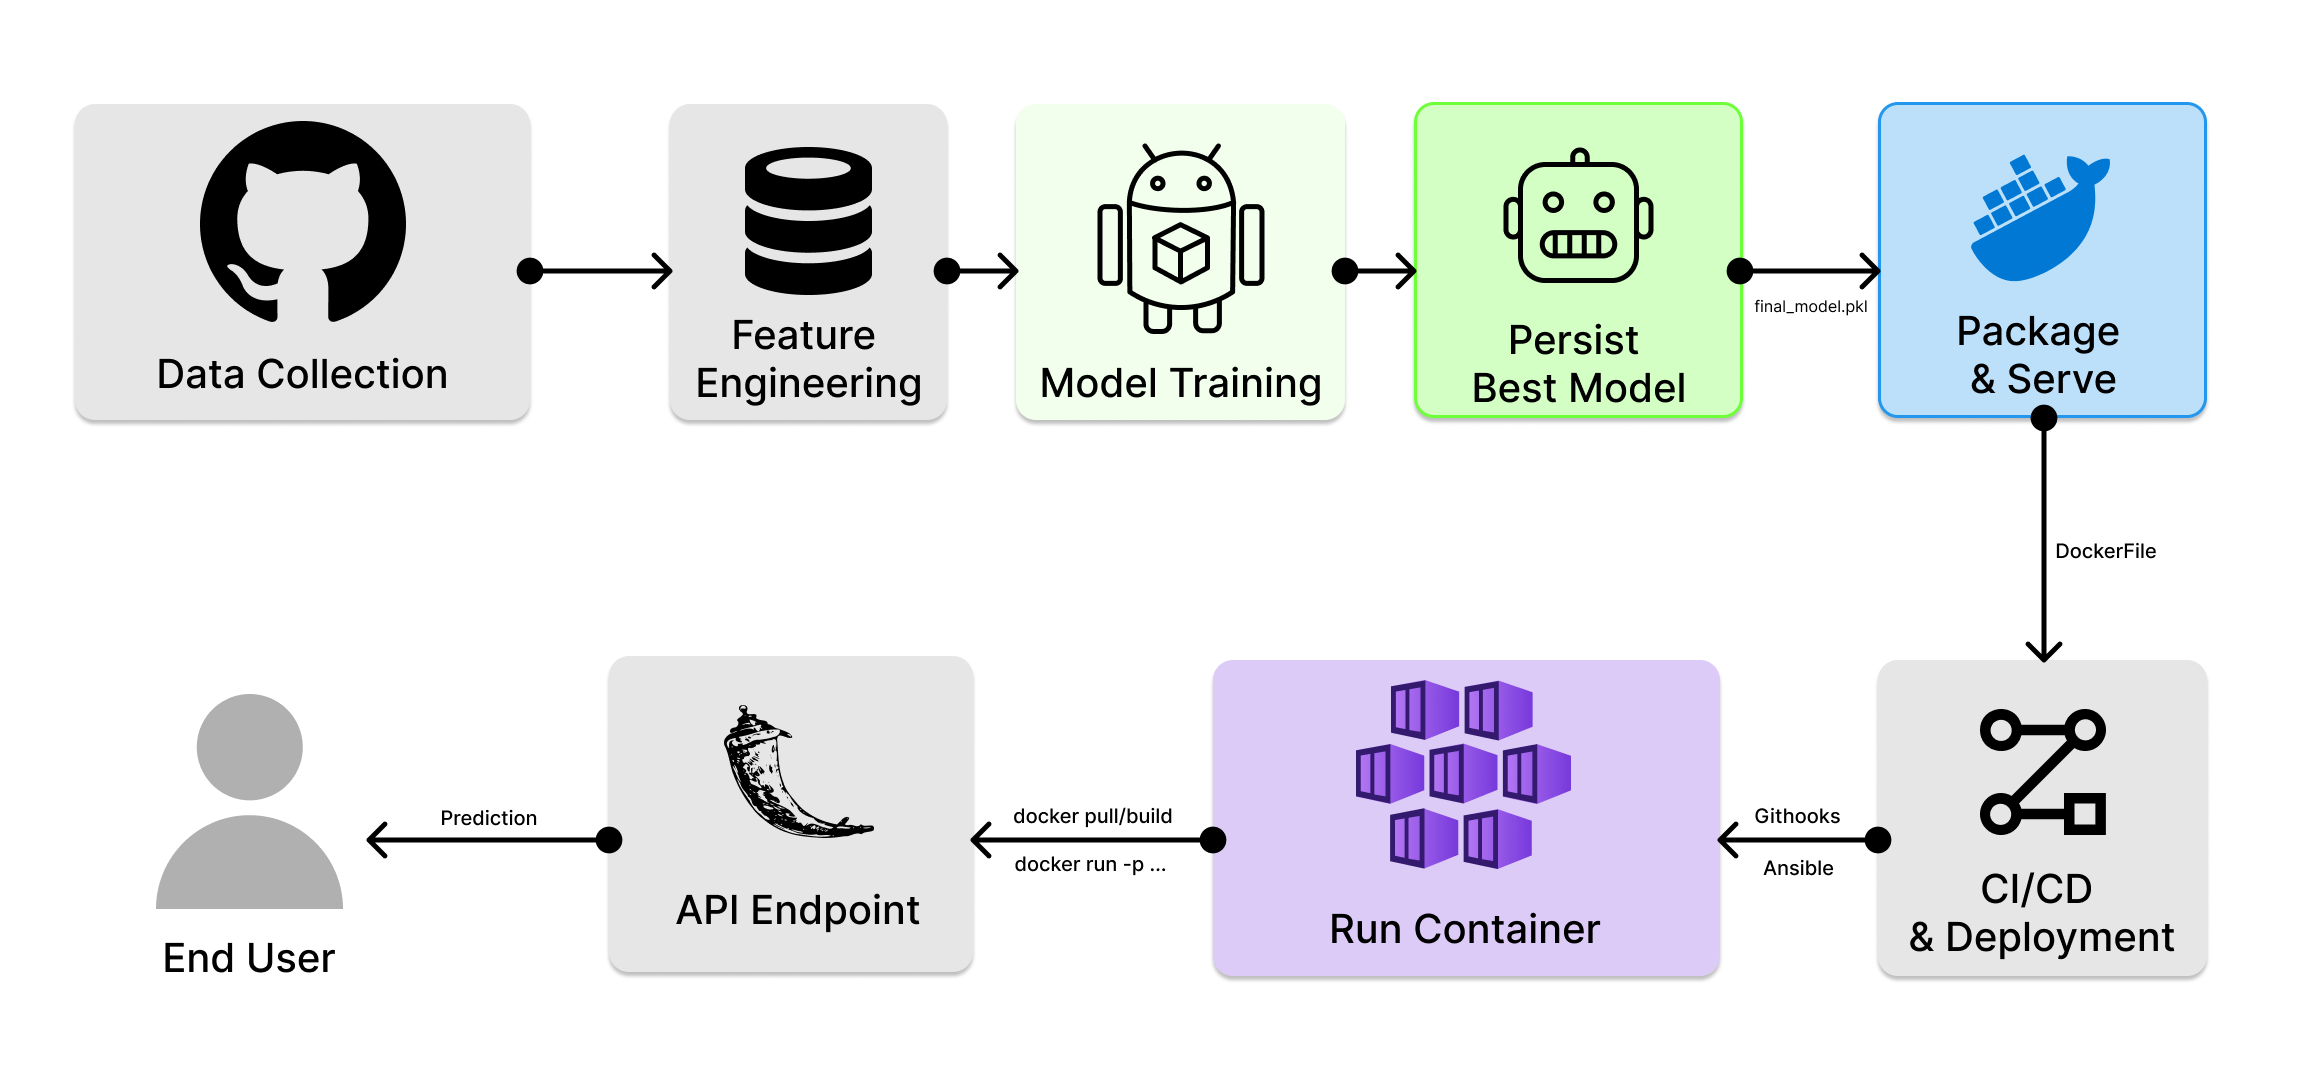
\includegraphics[width=0.8\textwidth]{Architecture.png}
  \caption{System Architecture}
  \label{fig:my-image}
\end{figure}

\section{Results}
\subsection{Scalability Analysis}
We studied the scalability of our project focusing first on the training time, we tried different combinations of VMs for ray tuning as explained later.
Vertical scaling: We increased computational resources by moving from 1 vCPU → 2 vCPU → 4 vCPU in a single VM, producing a roughly linear speed-up (218 s - 89 s - 40 s).
% Vertical Scaling Table
\begin{table}[ht]
  \centering
  \caption{Vertical Scaling: Single-VM Training Times}
  \label{tab:vertical_scaling}
  \begin{tabular}{l r}
    \toprule
    \textbf{VM Size (vCPU)} & \textbf{Training Time (s)} \\
    \midrule
    Small (1 vCPU)   & 218.35 \\
    Medium (2 vCPU)  &  89.97 \\
    Large (4 vCPU)   &  40.72 \\
    \bottomrule
  \end{tabular}
\end{table}

Horizontal (strong) scaling: We kept the VM size fixed (2 vCPU) but added more identical nodes. Doubling from 1 to 2 VMs halved the time (90 s → 40 s), and tripling to 3 VMs cut it to ~27 s—again near‐linear speedup.

% Horizontal Scaling Table
\begin{table}[ht]
  \centering
  \caption{Horizontal (Strong) Scaling: Training Time vs. Number of Medium VMs}
  \label{tab:horizontal_scaling}
  \begin{tabular}{r r}
    \toprule
     \textbf{Medium VMs (2 vCPU each)} & \textbf{Training Time (s)} \\
    \midrule
    1 Medium VM & 89.97 \\
    2 Medium VMs & 40.23 \\
    3 Medium VMs & 27.20 \\
    \bottomrule
  \end{tabular}
\end{table}


We also benchmarked the /predict endpoint of the deployed Flask application to evaluate how well the system handles real-time model inference under load. Using ApacheBench with 1000 POST requests and 10 concurrent users, the application maintained a throughput of 351.69 requests per second with zero failed requests. The median prediction response time was 28 ms, and the maximum was only 45 ms. These results demonstrate that the deployed model serves real-time predictions efficiently and reliably, making it scalable for multiple concurrent users in practical scenarios.

\begin{table}[H]
\centering
\caption{Load test results for \texttt{/predict} endpoint using ApacheBench}
\begin{tabular}{|l|c|}
\hline
\textbf{Metric} & \textbf{Value} \\
\hline
Requests completed         & 1000 \\
Failed requests            & 0 \\
Concurrency level          & 10 \\
Requests per second        & 351.69 \\
Mean time per request      & 28.43 ms \\
Max request time           & 45 ms \\
Median response time       & 28 ms \\
\hline
\end{tabular}
\label{tab:predict-benchmark}
\end{table}

Taken together, these numbers illustrate that our deployed model–serving stack is both fast and stable: it can sustain steady throughput at low per‐request latencies, with minimal variation between typical and worst‐case response times.

\begin{figure}[H]
  \centering
  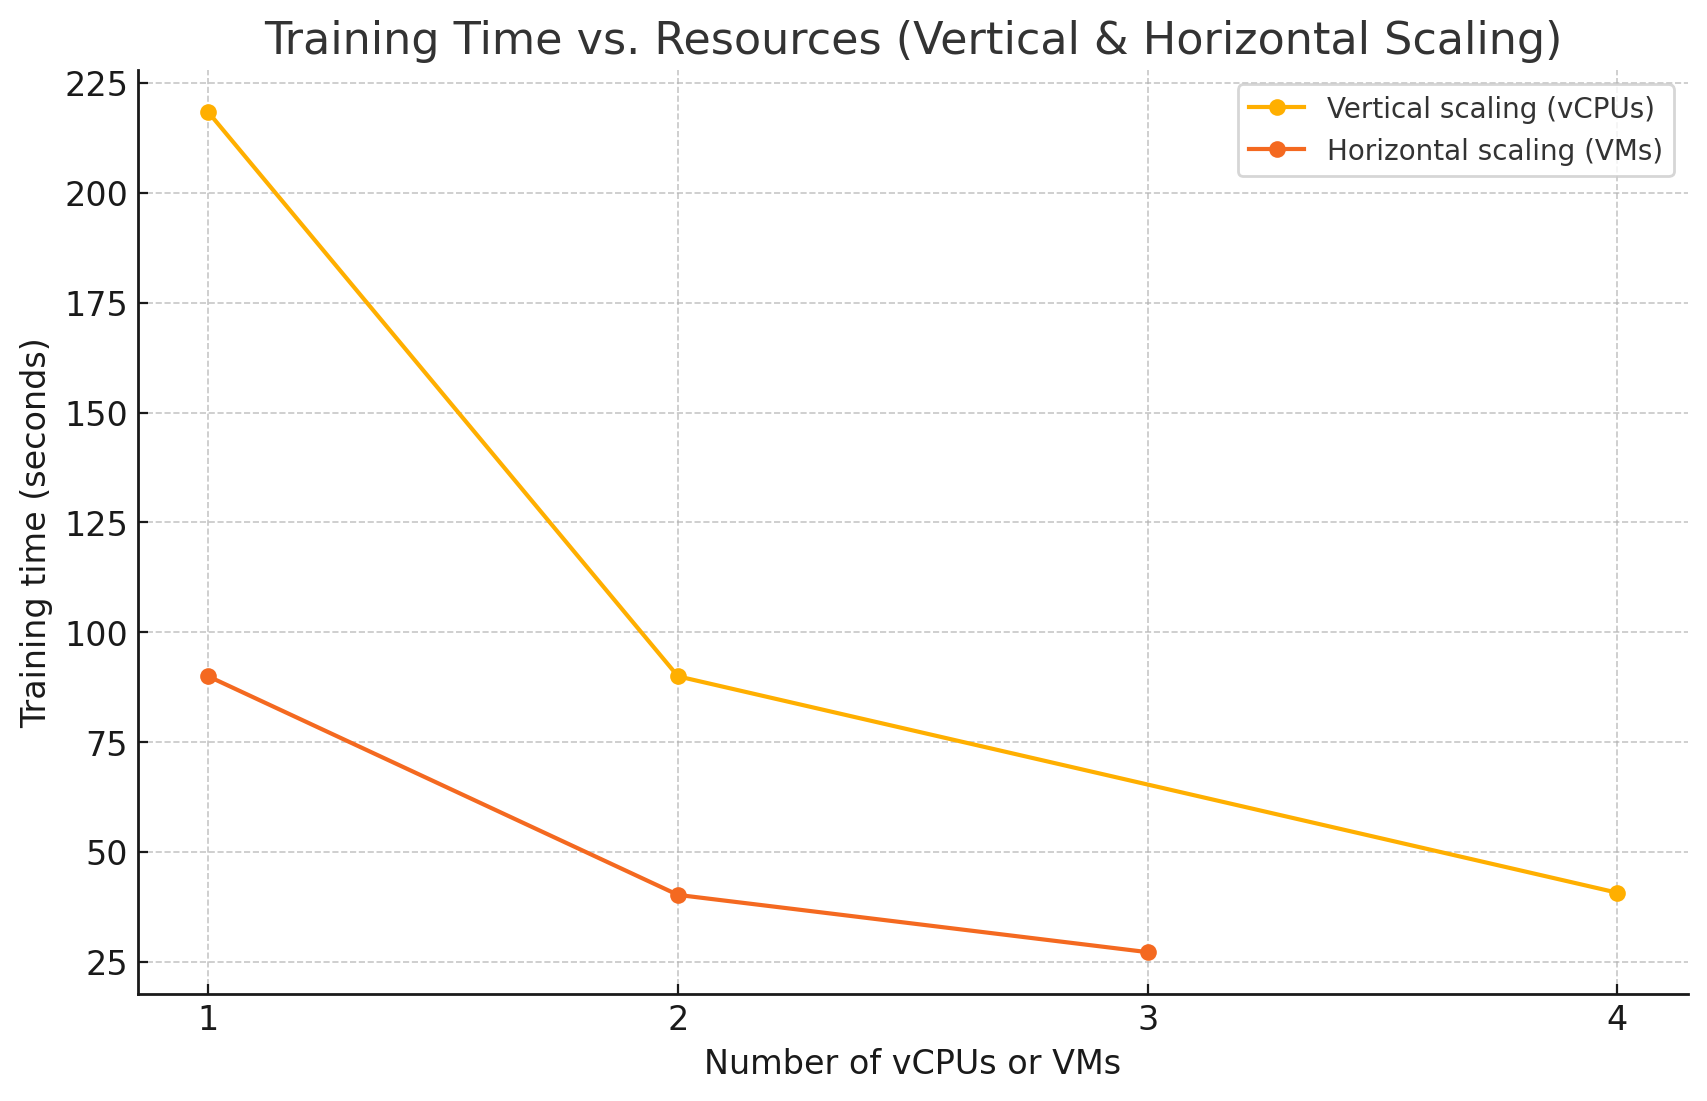
\includegraphics[width=0.7\textwidth]{Comparison.png}
  \caption{Scalability Comparison}
  \label{fig:my-image}
\end{figure}

\subsection{Model Comparison and Accuracy}
We evaluated five models:
\begin{itemize}[noitemsep]
    \item Linear Regression: R² = 0.54
    \item Ridge Regression: R² = 0.54
    \item Random Forest: R² = 0.50
    \item XGBoost: R² = 0.61
    \item LightGBM: R² = 0.59
\end{itemize}

The best performance was achieved using \textbf{XGBoost}, and it was exported as a `.pkl` artifact used in the deployed app. Predictions on real-world repositories showed close alignment with actual star counts, validating the generalization of the model.

\section{Conclusion}
We demonstrated an end-to-end predictive pipeline for estimating GitHub stars based on repository metadata. The system is modular, reproducible, and production-ready. Future extensions may include time-series forecasting or community activity trends to improve accuracy further. Additionally, active learning could be a valuable implementation to iteratively enhance the model by selectively querying the most informative data points 

\begin{thebibliography}{9}

\bibitem{1}
J. Han, S. Deng, X. Xia, D. Wang, and J. Yin,  
\textit{Characterization and prediction of popular projects on GitHub},  
In Proceedings of the 43rd IEEE Annual Computer Software and Applications Conference (COMPSAC), 2019, pp. 190--199.


\bibitem{2} L. Ren, S. Shan, X. Xu, and Y. Liu, \textit{StarIn: An Approach to Predict the Popularity of GitHub Repository}, Proc. 6th Int. Conf. of Pioneering Computer Scientists, Engineers and Educators (ICPCSEE 2020), 2020, pp. 258--273.

\bibitem{3}
H. Borges, A. Hora, and M. T. Valente,
\textit{Predicting the popularity of GitHub repositories},
In Proceedings of the 12th International Conference on Predictive Models and Data Analytics in Software Engineering, 2016, pp. 1--10.

\bibitem{4}
S. E. Sahin, K. Karpat, and A. Tosun,  
\textit{Predicting popularity of open source projects using recurrent neural networks},  
IEEE Access, vol. 7, pp. 149601--149615, 2019.

\end{thebibliography}



\end{document}